\documentclass{article}
\usepackage[utf8]{inputenc}
\usepackage[spanish]{babel}
\usepackage{listings}
\usepackage{graphicx}
\usepackage{hyperref}
\graphicspath{ {images/} }
\usepackage{cite}

\begin{document}

\begin{titlepage}
    \begin{center}
        \vspace*{1cm}
            
        \Huge

 \textbf{Parcial 2 - Informática II}
            
        \vspace{0.5cm}
        \LARGE
        
            
        \vspace{1.5cm}
            
        \textbf{Hecho por: \\\
        José Alejandro Moreno Mesa - C.C: 1001369765\\\
        Miguel Ángel Restrepo Rueda - C.C: 1001017183
        }
            
        \vfill
            
        \vspace{0.8cm}
            
        \Large
        Departamento de Ingeniería Electrónica y Telecomunicaciones\\
        Universidad de Antioquia\\
        Medellín\\
        Septiembre de 2021
            
    \end{center}
\end{titlepage}
\tableofcontents
\newpage
\section{ Análisis del problema y consideraciones para la alternativa de solución propuesta.}
La disposición del reto trae ciertos factores importantes a considerar:
\newline
1. El montaje del circuito que tenga una matriz de Neopixels de 8x8. 
2. La recepción de la imágen y cargarla correctamente en Qt.
\newline
3. Procesamiento correcto de la información de la imagen para saber su tamaño en pixeles.
\newline
4. Someter la información a un redimensionamiento para que pueda funcionar correctamente con el resto de la lógica y así sea mostrada eficazmente en tinkercad con las dimensiones correctas de una matriz de Neopixel de 8x8.
\newline
5. Hacer el análisis de los colores para los píxeles seleccionados del archivo original. Esto implica extraer el color de cada uno de los píxeles de la bandera recibida en JPG. 
\newline
6. Ordenar la información en un arreglo multidimensional.
\newline
7. Hacer el guardado en un archivo que pasará a Tinkercad.
Recibir la información en Tinkercad.
\newline
8. Copiar el código de Qt a Tinkercad. 
\newline
9. Mostrar los colores correctos en los LEDs RGB.
\newline
\newline
En primer lugar consideramos que solo es necesario una clase, llamada imagen, la cual contendrá los siguientes métodos, el primer método corresponde al constructor de la clase:
\newline
1. Qimage imagen(string nombre): Función que recibe el nombre de la imagen.jpg y que crea un objeto de la clase Qimage para su posterior regreso (return).
\newline
2.Submustreo y sobremuestreo.
\newline
3.void Arreglo(int ***original): Función que recibe un triple puntero que apunta a un arreglo de triple dimensión creado previamente. En ésta, se recorrerá el objeto de tipo Qimage devuelto por la función 1 para así organizar en orden sucesivo los datos RGB de cada uno de los píxeles de este y almacenarlos en el arreglo que se ingresó. En general, el arreglo tendrá una dimensión de tipo “Arreglo[8][8][3]”.
\newline
4.void Guardar(int ***original, string nombrearchivo): Función que recibe el triple puntero que apunta a la dirección en memoria del arreglo editado en la función 2 y que guarda su información en el archivo cuyo nombre es ingresado como el string llamado “nombrearchivo”.
\newline
5.En Tinkercad: void Mostrar(**original): Función que recibe la dirección del arreglo donde están los datos de los RGB de cada LED y que lo recorre para posteriormente mostrarlo en la “matriz de Neopixels” conectada en el circuito.
\newline
\newline
Por otro lado, los atributos de la clase imagen, serán: 
\newline
1. Ancho, que será para saber el ancho de la imagen proporcionado por el usuario, este atributo será necesario para hacer el redimensionamiento del ancho de la bandera.
\newline
2. Alto, que será para saber la altura de la imagen proporcionada por el usuario, este atributo será necesario para hacer el redimensionamiento de la altura  de la bandera.
\newline
3. Pixelsorig, que se usará para saber el total de píxeles de la imagen proporcionada por el usuario, este atributo será necesario para hacer el redimensionamiento de los pixels de la bandera para que concuerden con el circuito que contiene una matriz de Neopixels de 8x8.
\newline
4. Nombre, que será para saber el nombre de la imagen suministrada, esto es necesario para poder cargar la imagen de la bandera en Qt. 
\newline
5. ArregloRGB, este será un tiple puntero, en el que se guarde toda la información procesada, apuntará al arreglo con toda la información( el cual corresponde a un método de la clase). 

\newpage
\section{Esquema de las tareas definidad en el desarrollo del algoritmo}
Las tareas que consideramos necesarias para este proyecto son:
\newline
1. Montaje del circuito.
\newline
2. Pruebas del circuito (Para saber que todos los componentes están bien conectados, para se hace un ciclo for en el que se le manda 1 o en su defecto High a todos los Neopixels).
\newline
3. Creación en Qt de la clase ya descrita con sus respectivos métodos y atributos.
\newline
4. Prueba de la clase en Qt.
\newline
5.Paso del código de Qt a Tinkercad.
\newline
6. Ajuste del código en Tinkercad.
\newline
7. Pruebas finales.
\newline
8. Desarrollo de los informes.
\newline
9. Realización de los commits diarios. 
\newline
10. Realización del vídeo de YouTube, cumpliendo los requisitos dados en la guía del parcial 2. 
\newline
11. Entrega final.
\newline
12. Repaso del código y circuito implementado para poder hacer la sustentación.


\newpage
  \section{Algoritmo}
  
  \begin{figure}
  
  \centering
  
  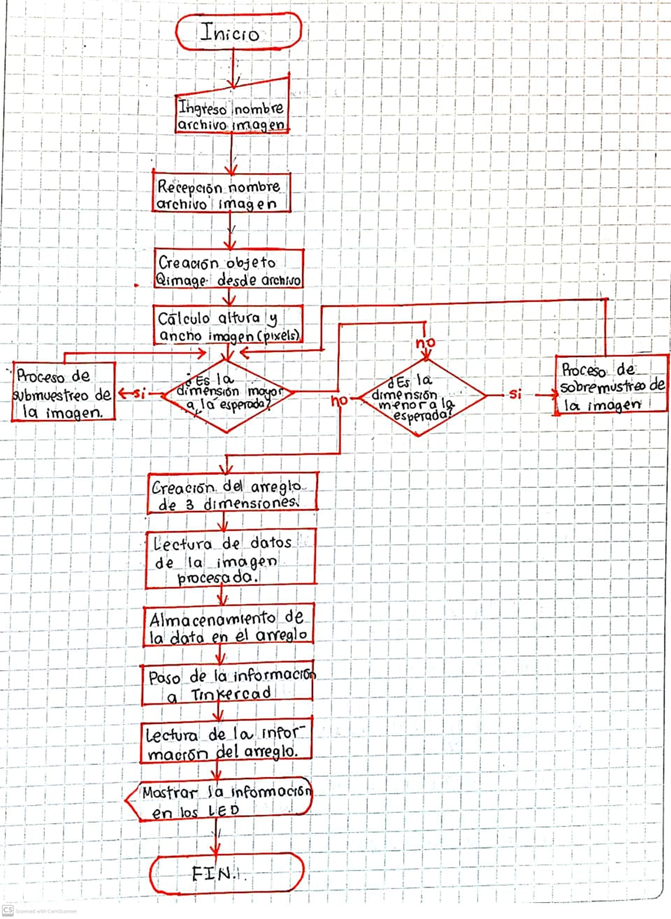
\includegraphics[width=1.3\textwidth]{Algoritmo.png}
  
  \caption{\label{fig1r}Algoritmo a implementar.}
  
  \end{figure}
  
\newpage
\section{Consideraciones a tener en cuenta en la implementación.}
Las consideraciones a tener en cuenta son las siguientes: 
\newline
1. Para montar el circuito, es mucho más fácil utilizar la tira de 8 Neopixels, de hecho también es más sencillo usar una matriz de 8x8 LEDs, ya que al tener una matriz con grandes dimensiones, el programa de Tinkercad sería muy pesado para procesar, lo que afecta la experiencia del usuario, además de que con una matriz 8x8 es más que suficiente para poder distinguir la bandera ingresada por el usuario.
\newline
2. Es necesario usar la librería Qimage, esto para cargar la imagen en Qt. 
\newline
3. Para el redimensionamiento de la imagen proporcionada, es necesario hacer sobremuestreo o submuestro, según sea el caso, para esto, pensamos obtener cuál sería el tamaño en pixeles de una matriz 8x8 de neopixels de Tinkercad, para luego coger la imagen inicial, analizar sus dimensiones, para ver qué tan grande o qué tan pequeña es en comparación con el tamaño de la matriz 8x8, al saber si es más grande o más pequeña que el tamaño de la matriz 8x8, se procede a hacer sobremuestreo o submuestro, según sea el caso, para esto, si es más grande la imagen que la matriz, se dividirá entre 2 la cantidad total de píxeles hasta que se acerque el número de píxeles al de la matriz, pero cuando se esté acercando al resultado, se entrará en un ciclo que terminará de redimensionar la imagen, ahora, cuando la imagen sea más pequeña que la matriz, se hará un procedimiento muy similar al anteriormente mencionado solo que, se multiplicará por 2 la cantidad total de píxeles.
\newline
4. En relación con el punto anterior, creemos que el submuestreo o sobremuestreo puede ser la parte más complicada del parcial, ya que, se puede tener casi que cualquier dimensión de imagen, por lo que el algoritmo ideado tiene que ser muy sólido, porque incluso de esto depende el resto del código.  
\newline
5. Para obtener el color de cada pixel de la imagen dada por el usuario, se indagará como aplicaciones ampliamente conocidas como Instagram, hacen esto, de hecho, nos apoyaremos en el aclamado software, paint, ya que este tiene muchas prestaciones a la hora de trabajar con imágenes.
\newline
6. Como es bien sabido, será necesario buscar la documentación de la librería Qimage, ya que esta será de gran utilidad para cargar las imágenes a Qt. 
\newline
7. Se incluirá la librería Fstream, esta para el manejo de strings, ya que es un tipo de dato que tiene muchas funciones ya implementadas, que nos ahorrarán mucho tiempo. 
\newline
8. Otra cosa a tener en cuenta que tiene mucha relevancia, es las banderas que tienen figuras en ellas, por ejemplo, la bandera de Japón, Brasil, Canadá entre otras, con las cuales hay que tener mucho cuidado ya que se tiene que mostrar correctamente las figuras contenidas en ellas en la matriz de Tinkercad. 



\end{document}
